\scanpage{31}
\mspage{16}
Si on considère le quotient \inserted{$N_{g,\nu}$} de $M_{g,\nu}$ par $\mathfrak S_\nu$ (de sorte que $M_{g,\nu}$ est un rev. de groupe $\mathfrak S_\nu$ de $N_{g,\nu}$) \unsure{on a|\ldots}
\diagram{\begin{tikzcd}[ampersand replacement=\&,column sep=small,row sep=small]
(5)\quad1 \arrow[r] \& \pi_1(\overline M_{g,\nu}) \arrow[r] \&
\pi_1(N_{g,\nu},\xi) \arrow[rr] \arrow[dr,phantom,"="] \arrow[dd,phantom,"\Vert"] \& \&
\mathfrak S_\nu\times\Gamma \arrow[r] \& 1\\
\& \& \& \pi_1(\overline N_{g,\nu},\Gamma;\unsure{\xi|j}) \arrow[d,phantom,"\Vert"]\\
\& \& \pi_1(M_{g,\nu},\mathfrak S_\nu,\xi) \arrow[r,phantom,"="] \&
\pi_1(\overline M_{g,\nu},\mathfrak S_\nu\times\Gamma)
\end{tikzcd}}
structure d'extension un peu plus riche que la première ligne de (4). La conjecture \unsure{faite|fait} équivaut \unsure{à|:} la suivante :
\[
\pi_1(N_{\unsure{g\nu|g,\nu}};\xi)\xrightarrow{\sim}\operatorname{Autextlac}\bigl(\pi_1(X_{\unsure{\xi|j}}\setminus\{x_1,\mathbin{-}x_\nu\})\bigr)
\]
ou encore
\[
\Gamma\simeq\operatorname{Autextlac}\bigl(\pi_1(X_{\unsure{\xi|j}}\setminus\{x_1,\mathbin{-}x_\nu\})\bigr)/\widetilde{\mathcal T}_{g,\nu}^{\wedge}
\]
où
\[
\widetilde{\mathcal T}_{g\nu}\simeq\operatorname{Autextlac}^{+}\bigl(\pi_1(X_{\unsure{\xi|j}}^{an}\setminus\{x_1,\mathbin{-}x_\nu\}).
\]

$*$ NB Il faudrait déterminer le groupe des automorphismes 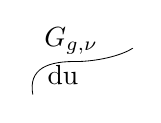
\begin{tikzpicture}[baseline=(base.base)]
\node[anchor=base west,inner sep=0] (base) at (0,0) {du};
\node[anchor=base west,inner sep=0] at (-.04,.48) {\inserted{$G_{g,\nu}$}};
\draw[line width=.3pt] (-.18,-.13) .. controls (-.24,.20) and (.01,.30) .. (.40,.29) .. controls (.70,.30) and (.97,.38) .. (1.09,.46);
\end{tikzpicture} topos modulaire géom $\overline M_{g,\nu}$ \deleted{\unsure{est}} ($G_{g,\nu}=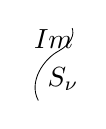
\begin{tikzpicture}[baseline=(base.base)]
\node[anchor=base west,inner sep=0] (base) at (0,0) {$\mathfrak S_\nu$};
\node[anchor=base west,inner sep=0] at (-.17,.48) {$\inserted{\operatorname{Im}}$};
\draw[line width=.3pt] (-.11,-.18) .. controls (-.24,.06) and (-.04,.35) .. (.15,.45) .. controls (.31,.54) and (.35,.66) .. (.32,.74);
\end{tikzpicture}$ ? \unsure{\deleted{)}|\}} Sans doute $\mathfrak S_\nu$ opère fidèlement sauf $g=0,\nu\leq4$\textendash\,\textemdash)

\uline{Question}
\[
\Gamma\longrightarrow\operatorname{Autext}\,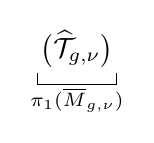
\begin{tikzpicture}[baseline=(arg.base)]
\node[inner sep=1pt] (arg) {$\bigl(\widehat{\mathcal T}_{g,\nu}\bigr)$};
\draw ([yshift=-1pt]arg.south west) -- ([yshift=-5pt]arg.south west) --
      ([yshift=-5pt]arg.south east) -- ([yshift=-1pt]arg.south east);
\node[anchor=north,inner sep=1pt] at ([yshift=-5pt]arg.south)
      {$\scriptstyle\pi_1(\overline M_{g,\nu})$};
\end{tikzpicture}
\quad\left\{\begin{array}{l}\text{injectif ?}\\\text{bijectif}\end{array}\right.
\]
\margin{(Sans doute il faut condition \unsure{sur le} \illegible{1}, cf NB.}
\mspage{30}
